\section{Patterns 3 - GoF Factory Method/Astarct Factory}

\subsection{Fokuspunkter}

\begin{itemize}
	\item Redegør for, hvad et software design pattern er.
	\item Redegør for opbygningen af GoF Factory Method og GoF Abstract Factory.
	\item Giv et designeksempel på anvendelsen af GoF Abstract Factory.
	%\item Redegør for opbygningen af GoF Singleton.
	%\item Redegør for fordele og ulemper ved anvendelsen af GoF Singleton
\end{itemize}

\subsection{Hvad er et Software pattern?}

\derp

\subsection{Redegør for opbygningen af GoF Factory Method}

\textit{''Define an interface for creating an object, but let subclasses decide which class to instantiate. The Factory method lets a class defer instantiation it uses to subclasses''}

\begin{figure}[H]
	\centering
	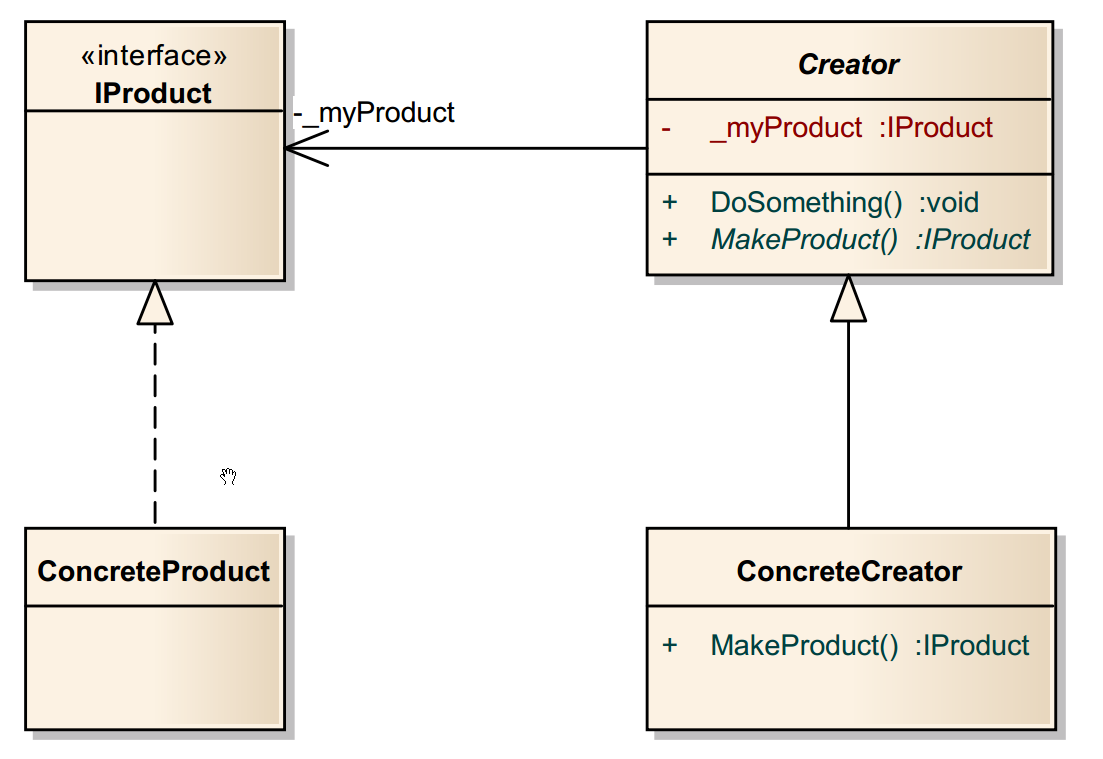
\includegraphics[width=0.6\linewidth]{figs/facmet}
	\caption{Klassediagram for FactoryMethod}
	\label{fig:facmet}
\end{figure}

Omkring selve implementeringen af en klasse m.m. som bruger factory method kan listing~\ref{code:factorymethod} ses:

\begin{lstlisting}[
caption=Realisering og brug af factory method.,
label=code:factorymethod]
public abstract class Creator
{
	// IProduct to be used for stuff
	IProduct _myProduct;
	
	// ctor eller anden nyttig function?
	public void DoSomething()
	{
		_myProduct = MakeProduct();
		Console.WriteLine(_myProduct.GetType().Name + " says hello!");
	}

	// Factory method -> to be implemented in subclass...
	public abstract IProduct MakeProduct();
}

public class ConcreteCreator : Creator
{
	public override IProduct MakeProduct()
	{
		// returns some subclass of IProduct
		return new ConcreteProduct();
	}
}
\end{lstlisting}

\subsection{Redegør for opbygningen af GoF Abstract Factory}
Hvis man har et klassediagram som ser ud noget i stil med det på figur~\ref{fig:compressionstockings_classdiagram} og en main ligner noget ala det i listing~\ref{code:compressionmain} så står det meget hurtigt en klart at dette er meget rodet og uoverskueligt. For at undgå disse babushka dukker bliver løsningen \textbf{Abstract Factory} og denne er beskrevet under figur og kode.

\begin{figure}[H]
	\centering
	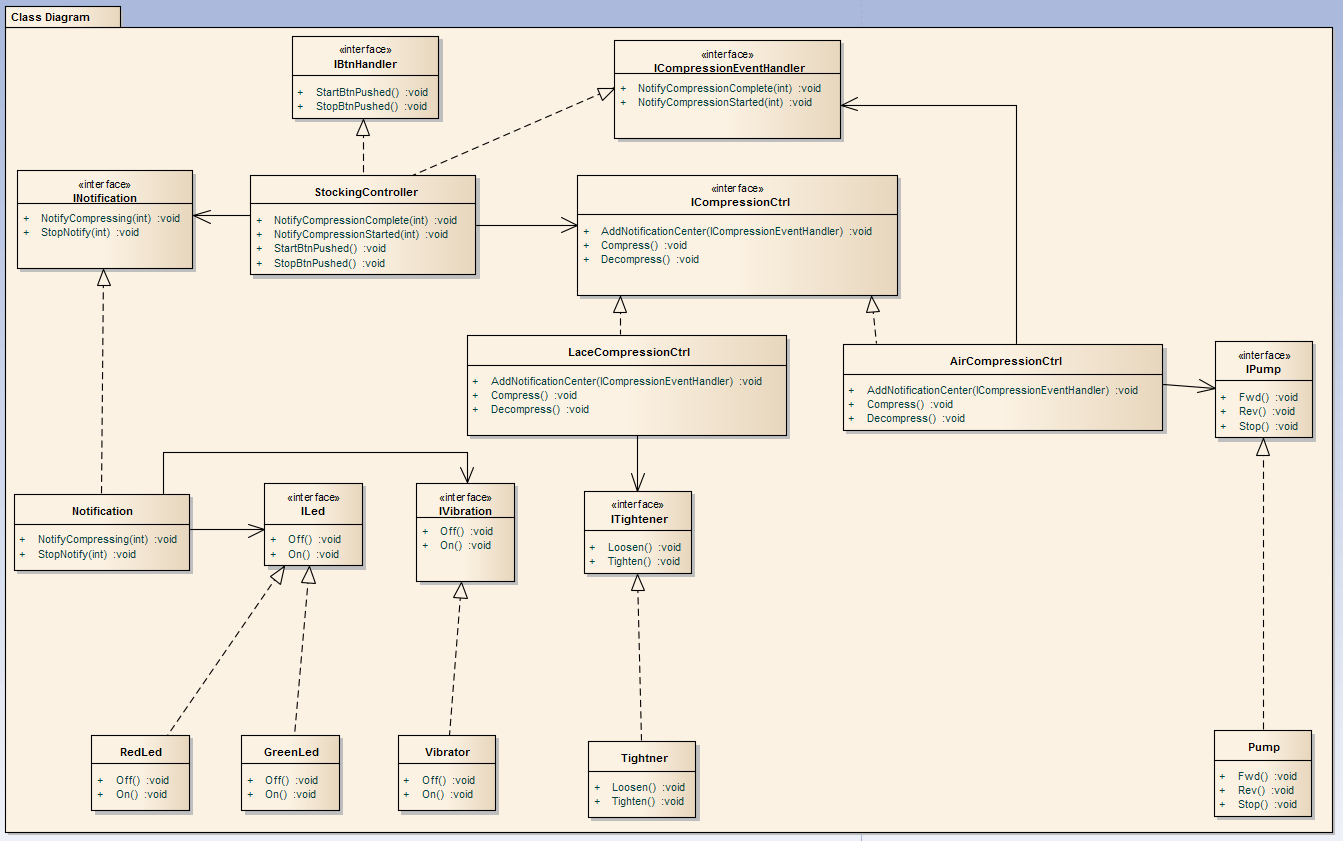
\includegraphics[width=0.9\linewidth]{figs/compressionstockings_classdiagram}
	\caption{Klassediagram for compressionstocking systemet.}
	\label{fig:compressionstockings_classdiagram}
\end{figure}

\begin{lstlisting}[caption=Main for compressionstocking.application.,
label=code:compressionmain,
morekeywords={INotificationDevice,ICompressionCtrl,IButtonHandler}]
IPump myPump = new Pump();
ITightner myTightner = new Tightner();
ICompressionCtrl myCompressionCtrl = new LaceCompressionCtrl(myTightner);

INotificationDevice myGreenLed = new LedGreen();
INotificationDevice myReDevice = new LedRed();
INotificationDevice myVibrator = new Vibrator();
INotification myNotification = new Notification(myGreenLed, myReDevice, myVibrator);

IButtonHandler myStockingCtrl = new StockingCtrl(myCompressionCtrl, myNotification);
myCompressionCtrl.AddNotificationCenter(myEventHandler);
\end{lstlisting}



\subsection{Giv et designeksempel på anvendelsen af GoF Abstract Factory}
\todo{classdia}